\subsubsection{DBScan Modell}
\label{subsubsec:dbscan}
Die erste Idee nach dem Basismodell, um ähnliche Hotels zu finden, ist es den weitverbreiteten \emph{Density-Based Spatial Clustering of Applications with Noise-Algorithmus} zu nutzen. Der \emph{Density-Based Spatial Clustering of Applications with Noise-Algorithmus} kurz DBScan ist ein leistungsfähiger Ansatz zur Clusteranalyse, der darauf abzielt, Cluster in Datensätzen mit variabler Dichte zu identifizieren. Anders als klassische Clustering-Algorithmen, die auf geometrischen Formen oder Distanzmetriken basieren, nutzt DBScan die Dichte der Datenpunkte, um Cluster zu identifizieren \cite{6814687}.
\newline
\newline
Die Identifikation von Clustern innerhalb eines Datensatzes erfordert vom DBScan-Algorithmus zwei wesentliche Informationen:

\begin{itemize}
    \item Mindestanzahl an Datenpunkten für die Bildung eines Clusters.
    \item Maximale Entfernung, in der Datenpunkte voneinander liegen dürfen.
\end{itemize}

Ein Vorteil des DBScan-Algorithmus besteht darin, dass keine vorherige Festlegung darüber getroffen werden muss, wie viele Cluster am Ende resultieren sollen. Es genügt die Angabe dieser beiden genannten Informationen, um die Bildung von Clustern zu ermöglichen.
\newline
\newline
Die zugrunde liegende Hypothese dieser Methodik besagt, dass der DBScan-Algorithmus alle ähnlichen Hotels in einem Cluster zusammenführt.

\paragraph{Vorbereitung des Datensatzes} 
Der in Abbildung \ref{img:all_features_4} dargestellte Datensatz enthält sowohl numerische als auch kategoriale Daten. Da der DBScan-Algorithmus ausschließlich mit numerischen Daten arbeiten kann, ist es erforderlich, den vorhandenen Datensatz vor der Anwendung des Algorithmus zu transformieren. Zu diesem Zweck wird eine Pipeline erstellt, die auf den gesamten Datensatz angewendet wird. In einem ersten Schritt werden die kategorialen Daten mithilfe von \emph{One-Hot-Encoding} umgewandelt. Darüber hinaus erfolgt eine Skalierung der bereits vorhandenen numerischen Daten.
\newline
\newline
Die Struktur der Pipeline ist wie folgt:

\begin{lstlisting}[language=Python, label=lst:pipeline, caption=Datensatz Pipeline]
from sklearn.compose import ColumnTransformer
from sklearn.pipeline import make_pipeline
from sklearn.preprocessing import StandardScaler, OneHotEncoder

numerical_features = ['median_min', 'median_max']
categorical_features = ['art', 'region2']
    
numerical_pipeline = make_pipeline(StandardScaler())
    
categorical_pipeline = make_pipeline(OneHotEncoder())
    
preprocessor = ColumnTransformer(
    transformers=[
        ('num', numerical_pipeline, numerical_features),
        ('cat', categorical_pipeline, categorical_features)
    ])
    
    
pipeline = make_pipeline(preprocessor)
\end{lstlisting}

Die in dem Listing \ref{lst:pipeline} gezeigte Pipeline kann nun auf Datensatz angewendet werden. Dazu muss die Pipeline zunächst du den Datensatz abgestimmt werden, um dann den Datensatz zu Transformieren. Dies wird mit dem folgenden Listing veranschaulicht:

\begin{lstlisting}[language=Python, label=lst:pipeline2, caption=Ausführung der Pipeline auf dem Datensatz]
# Anpassen der Daten an die Pipeline
pipeline.fit(df)

# Transformieren der Daten
transformed_df = preprocessor.transform(df)

# Erstelle einen DataFrame aus den transformierten Daten
model_df = pd.DataFrame(transformed_df.toarray(), 
                        columns=numerical_features + 
                            list(preprocessor.named_transformers_['cat']
                                                .named_steps['onehotencoder']
                                                .get_feature_names_out(categorical_features)))
\end{lstlisting}

\paragraph{Modellbildung} 
Nach erfolgter Transformation des Datensatzes kann dieser in den DBScan-Algorithmus eingegeben werden, um die Cluster zu generieren. Als Mindestanzahl an Datenpunkten für ein Cluster wird der Wert 2 festgelegt, da stets Paare von zwei Hotels gefunden werden sollen. Das Auffinden der Cluster erfolgt daraufhin lediglich durch einen Aufruf.

\begin{lstlisting}[language=Python, label=lst:dbscan, caption=Ausführung des DBScan-Algorithmus]
from sklearn.cluster import DBSCAN

# Define variables
eps = 0.8
min_samples = 2 

# Create the DBScan algorithm
dbscan = DBSCAN(eps=eps, min_samples=min_samples)

# Add Cluster to df
model_df['Cluster'] = dbscan.fit_predict(model_df)
\end{lstlisting}

Das Listing \ref{lst:dbscan} veranschaulicht die Initialisierung des DBScan-Algorithmus sowie die Erzeugung der individuellen Cluster. Diese Cluster werden anschließend der Datenreihe in der Spalte \emph{Cluster} zugeordnet.
\newline
\newline
In einem nachfolgenden Schritt können die erstellten Cluster wie folgt visualisiert werden:

\begin{figure}[h]
    \centering
    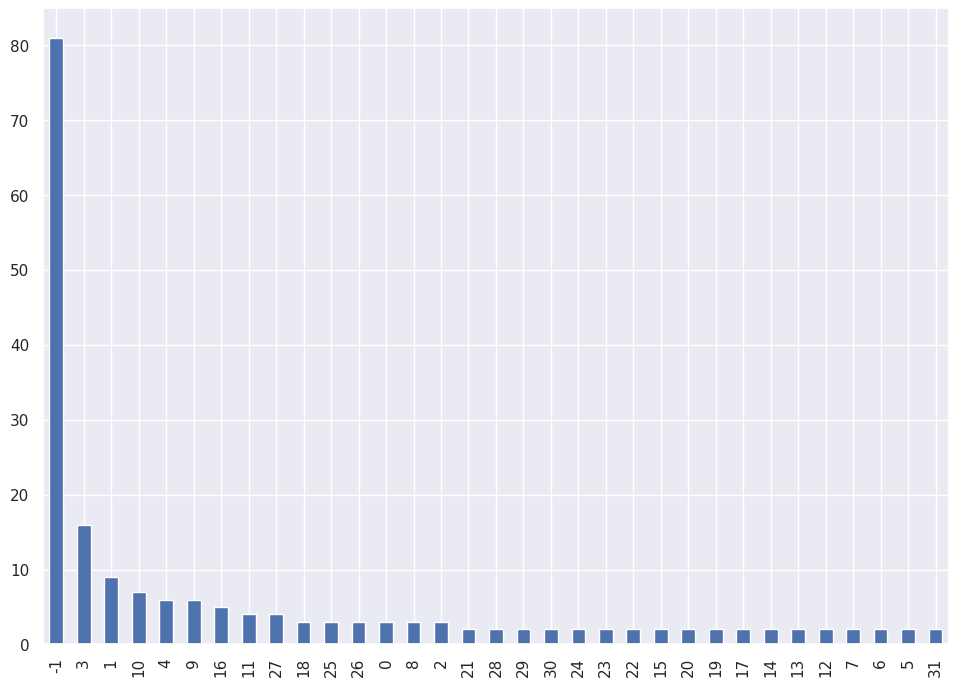
\includegraphics[width=0.85\textwidth, center]{cluster.png}
    \caption[DBScan Clusters]{DBScan Clusters}
    \label{img:cluster}
\end{figure}

Abbildung \ref{img:cluster} zeigt die verschiedenen Cluster, die durch den DBScan-Algorithmus erstellt wurden. Es sind insgesamt 32 Cluster zu erkennen, beginnend mit Cluster 0, sowie eine weitere Kategorie \emph{-1}, die anzeigt, dass für diese Hotels kein Cluster gefunden wurde. Bemerkenswert ist dabei, dass die Mehrheit dieser Hotels keinem Cluster zugeordnet wurde.
\newline
\newline
Ungeachtet dieser Beobachtung soll im nächsten Schritt überprüft werden, welche Hotels mit dem Benchmark-Hotel in einem Cluster vorhanden sind. Hierfür müssen die Hotel-IDs in einer zusätzlichen Spalte dem Dataframe hinzugefügt werden. Die nachfolgende Code-Sequenz im angegebenen Listing ermöglicht die Identifikation der Hotels, die mit dem Benchmark-Hotel in einem Cluster sind.

\begin{lstlisting}[language=Python, label=lst:dbscan_values, caption=Finden alle Hotel ID´s innerhalb des gleichen Clusters]
# Add hotel ids to the dataset with the clusters
model_df['hotel_id'] = df.index

# Get the row for the benchmark hotel
benchmark_row = model_df[model_df["hotel_id"] == str(benchmark_hotel_id)]

# Get the Cluster value of the benchmark hotel
benchmark_cluster = list(benchmark_row["Cluster"].values)[0]

# Get the rows with the same cluster as the benchmark hotel
benchmark_cluster_df = model_df[model_df["Cluster"] == benchmark_cluster]

# Get the hotel ids 
hotel_ids = list(benchmark_cluster_df["hotel_id"].values)
\end{lstlisting}

Die Variable \emph{hotel\_ids} enthält nun sämtliche Hotel-IDs, die zusammen mit dem Benchmark-Hotel in einem Cluster verortet sind. Initial besteht das Interesse darin, die identifizierten Hotels zu visualisieren. Daher soll im Anschluss angezeigt werden, welche Merkmale die identifizierten Hotels aufweisen.

\begin{figure}[h]
    \centering
    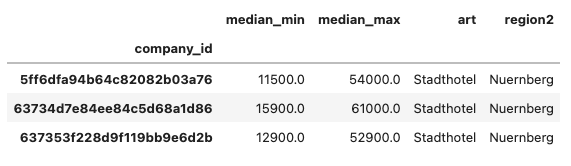
\includegraphics[width=1\textwidth, center]{dbscan_hotels_1.png}
    \caption[Gefundene Hotels für das erste Benchmark-Hotel mit dem DBScan-Algorithmus]{Gefundene Hotels für das erste Benchmark-Hotel mit dem DBScan-Algorithmus}
    \label{img:dbscan_hotels_1}
\end{figure}

Die Hotels, die im identifizierten Cluster zu finden sind, weisen tatsächlich Ähnlichkeiten zu den Merkmalen auf, die das Benchmark-Hotel mit der ID \emph{5ff6dfa94b64c82082b03a76} charakterisieren. Da die Aussagekraft eines einzelnen Hotels begrenzt ist, soll das zweite Benchmark-Hotel ebenfalls mit einbezogen werden. Hierbei sollen auch für dieses Hotel zunächst die identifizierten Hotels anhand ihrer Merkmale bewertet werden.

\begin{figure}[h]
    \centering
    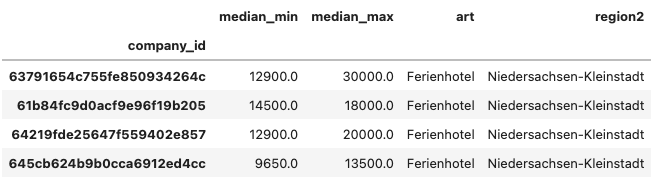
\includegraphics[width=1\textwidth, center]{dbscan_hotels_2.png}
    \caption[Gefundene Hotels für das zweite Benchmark-Hotel mit dem DBScan-Algorithmus]{Gefundene Hotels für das zweite Benchmark-Hotel mit dem DBScan-Algorithmus}
    \label{img:dbscan_hotels_2}
\end{figure}

Unter Berücksichtigung des zweiten Hotels wird ersichtlich, dass der DBScan Hotels mit ähnlichen Merkmalen identifiziert. Dennoch lässt sich anhand der vorliegenden Merkmale nicht eindeutig feststellen, ob diese Hotels tatsächlich ähnliche Verläufe in Bezug auf den RevPAR aufweisen.

\paragraph{Evaluation}
Angesichts der Tatsache, dass allein anhand der Merkmale keine klare Aussage über die tatsächliche Ähnlichkeit der Hotels getroffen werden kann, erfolgt in der nachfolgenden Sektion eine Evaluierung der beiden Benchmark-Hotels. 
\newline
\newline
Der Beginn dieser Evaluierung erfolgt mit dem Hotel, das die ID \emph{5ff6dfa94b64c82082b03a76} trägt. Die Ergebnisse dieser Evaluation werden im Folgenden dargestellt:

\begin{figure}[h]
    \centering
    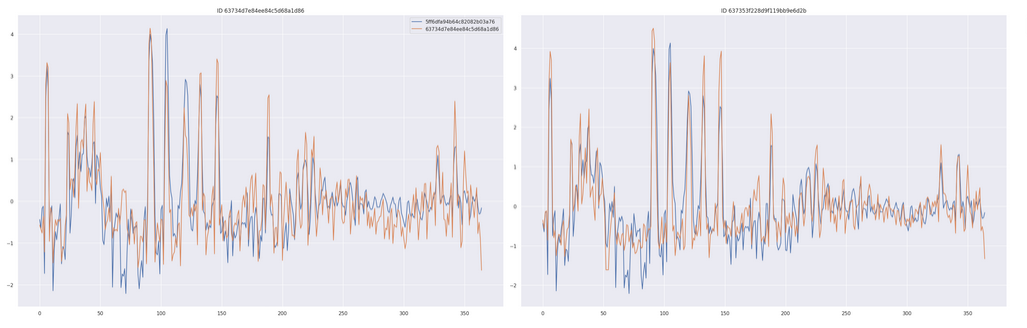
\includegraphics[width=1\textwidth, center]{dbscan_results_1.png}
    \caption[DBScan Ergebnisse der RevPAR-Verläufe für das erste Benchmark-Hotel]{DBScan Ergebnisse der RevPAR-Verläufe für das erste Benchmark-Hotel}
    \label{img:dbscan_results_1}
\end{figure}

\begin{figure}[h]
    \centering
    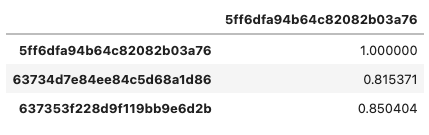
\includegraphics[width=1\textwidth, center]{dbscan_results_1_1.png}
    \caption[DBScan Ergebnisse der RevPAR-Korrelationen für das erste Benchmark-Hotel]{DBScan Ergebnisse der RevPAR-Korrelationen für das erste Benchmark-Hotel}
    \label{img:dbscan_results_1_1}
\end{figure}

Die Abbildungen \ref{img:dbscan_results_1} und \ref{img:dbscan_results_1} verdeutlichen, dass die identifizierten Hotels die Voraussetzungen für einen Korrelationswert von mindestens 0,8 erfüllen. Die Ergebnisse für das Hotel mit der ID \emph{5ff6dfa94b64c82082b03a76} erweisen sich demnach als zufriedenstellend. Allerdings ist eine gewisse Skepsis angebracht, da es auch rein zufällig sein könnte, dass diese Hotels Ähnlichkeiten in Bezug auf den RevPAR Verlauf aufweisen. Aus diesem Grund soll die gleiche Evaluation auch mit dem zweiten Hotel, welches die ID \emph{645cb624b9b0cca6912ed4cc} trägt, durchgeführt werden.

\begin{figure}[h]
    \centering
    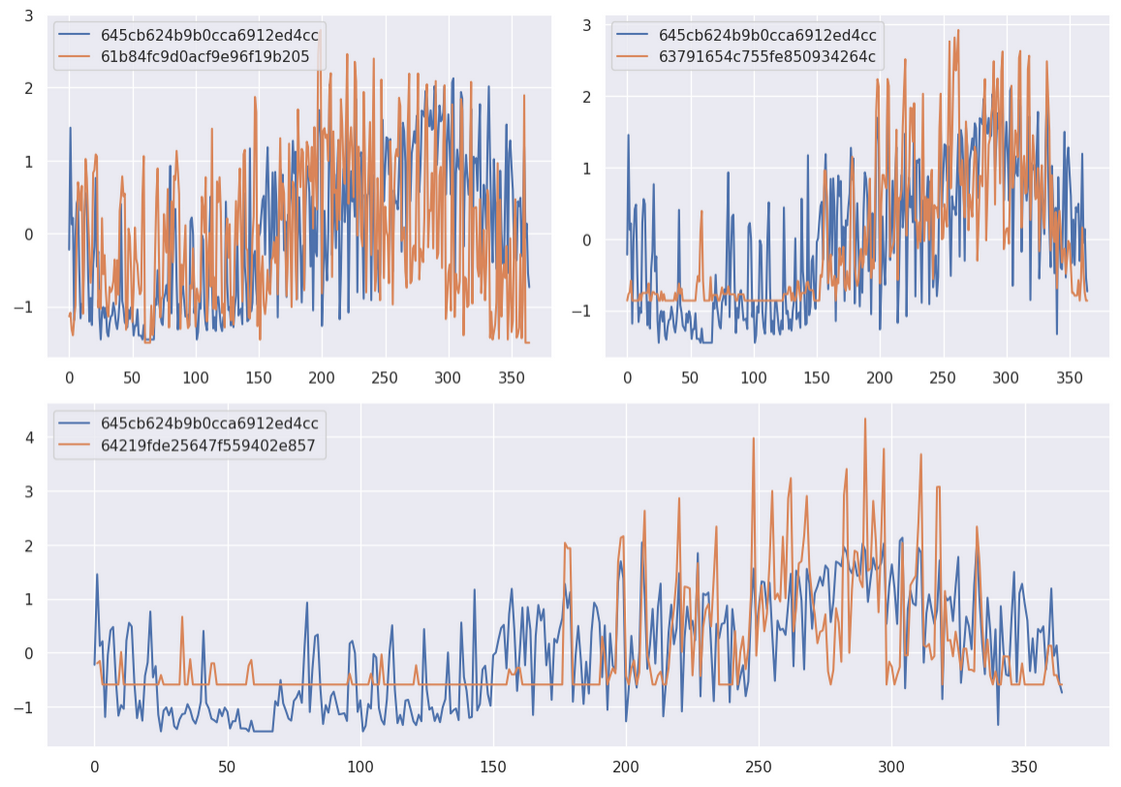
\includegraphics[width=1\textwidth, center]{dbscan_results_2.png}
    \caption[DBScan Ergebnisse der RevPAR-Verläufe für das zweite Benchmark-Hotel]{DBScan Ergebnisse der RevPAR-Verläufe für das zweite Benchmark-Hotel}
    \label{img:dbscan_results_2}
\end{figure}

\begin{figure}[h]
    \centering
    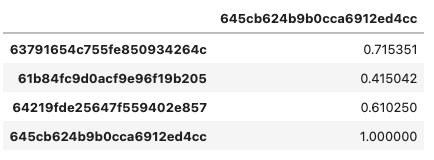
\includegraphics[width=1\textwidth, center]{dbscan_results_2_1.png}
    \caption[DBScan Ergebnisse der RevPAR-Korrelationen für das zweiten Benchmark-Hotel]{DBScan Ergebnisse der RevPAR-Korrelationen für das zweite Benchmark-Hotel}
    \label{img:dbscan_results_2_1}
\end{figure}

Die Evaluation des Hotels mit der ID \emph{645cb624b9b0cca6912ed4cc} ergab, dass die Anforderungen an einen Korrelationswert von mindestens 0,8 nicht erfüllt wurden. Somit lässt sich ableiten, dass die Ähnlichkeit der Merkmale zwischen den einzelnen Hotels nicht zwangsläufig mit der Ähnlichkeit in Bezug auf die RevPAR-Werte in Verbindung steht. 
\newline
\newline
Obwohl der DBScan-Algorithmus im Vergleich zum Basismodell verbesserte Ergebnisse lieferte, bleibt das Gesamtergebnis dennoch unbefriedigend. Besonders bedenklich ist dabei, dass die überwiegende Mehrheit der Hotels keinem Cluster zugeordnet werden konnten.

